%Included libraries
\documentclass[landscape,twocolum,letterpaper]{article}
\usepackage{graphicx}
\usepackage[margin=1.4cm]{geometry}
\usepackage{paralist}
\usepackage{chemformula}
\setlength{\columnseprule}{0.8pt}
\usepackage{soul,color}
\usepackage{multicol}
\usepackage{caption}
\usepackage{tabularx}
\usepackage{booktabs}
\usepackage[document]{ragged2e}
\usepackage{gensymb}
\usepackage{color, colortbl}
\definecolor{Gray}{gray}{0.9}
\newenvironment{Figure}
	{\par\medskip\noindent\minipage{\linewidth}}
		{\endminipage\par\medskip}
\usepackage{lipsum}
\usepackage{tikz}
\usetikzlibrary{shapes.geometric, arrows}
\newcommand\tab[1][1cm]{\hspace*{#1}}
\usepackage{tikz}
\usepackage{pagecolor}
%flow chart declarations
\tikzstyle{box} = [rectangle, rounded corners, minimum width = 1cm, minimum height=1cm,text justified, text width=8cm, draw=black, fill=white]
\tikzstyle{bar} = [rectangle, minimum width=30cm, minimum height=1cm, draw=white, fill=blue!20]
\tikzstyle{dia} = [diamond, minimum width=1cm, minimum height=0.4cm, text centered, draw=black, fill=green!30]
\tikzstyle{arrow} = [thick,->,>=stealth]
%Title and authors
\begin{document}
%need to include the Clemson Seal somewhere.
\center
\fontsize{18}{18}\selectfont{\textbf{Widespread Genotype-Phenotype Correlations in Intellectual Disability Associated with Specific Comorbidities and Secondary Clinical Phenotypes}}\\
\fontsize{8}{8}\selectfont{Zachary Gerstner$^1$, Emily L. Casanova$^{2,3}$, Julia L. Sharp$^4$, Manuel F. Casanova$^{2,3}$, Alex Feltus$^1$}\\
\centering
\begin{compactenum}
	\item Department of Genetics and Biochemistry, Clemson University, Clemson, South Carolina, USA
	\item Department of Biomedical Sciences, University of South Carolina Medical School at Greenville, South Carolina, USA
	\item Department of Pediatrics, Greenville Health System, Greenville, South Carolina, USA
	\item Department of Statistics, Colorado State University, Fort Collins, Colorado, USA
\end{compactenum}
%Goals

\begin{tikzpicture}
\node (start) [bar] {};
\end{tikzpicture}
\begin{multicols*}{3}
\flushleft
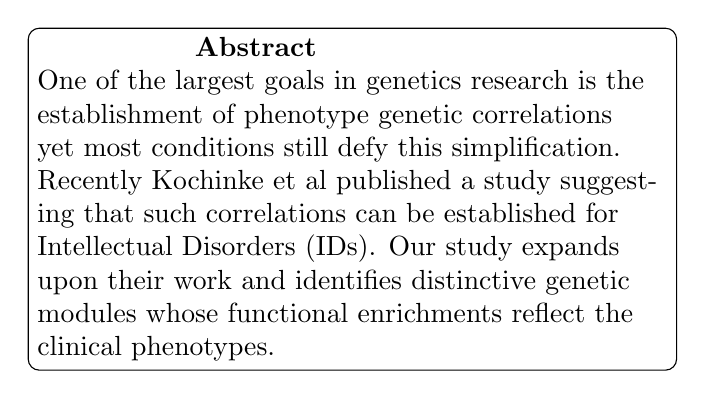
\begin{tikzpicture}[node distance=1cm]
\node (start) [box] {\tab \tab \selectfont{\textbf{Abstract}} \\ One of the largest goals in genetics research is the establishment of phenotype genetic correlations yet most conditions still defy this simplification. Recently Kochinke et al published a study suggesting that such correlations can be established for Intellectual Disorders (IDs). Our study expands upon their work and identifies distinctive genetic modules whose functional enrichments reflect the clinical phenotypes.};
\end{tikzpicture}
\fontsize{12}{12}\selectfont{\textbf{Abstract}}\\
\fontsize{10}{10}\selectfont{\tab One of the largest goals in genetics research is the establishment of phenotype genetic correlations yet most conditions still defy this simplification. Recently Kochinke et al published a study suggesting that such correlations can be established for Intellectual Disorders (IDs). Our study expands upon their work and identifies distinctive genetic modules whose functional enrichments reflect the clinical phenotypes. }\\
\justify
%Gene curation
%\fontsize{12}{12}\selectfont{\textbf{Methods}}
%\begin{tikzpicture}[node distance=2.5cm]
%\node (start) [box] {OMIM};
%\node (next1) [dia, right of=start] {Seed Genes};
%\node (next2) [box, right of=next1] {GeneMANIA};
%\node (next3) [dia, below of=next2] {Interactions};
%\node (next4) [box, left of=next3] {Cytoscape};
%\node (stop) {dia, right of=next4] {Final network};
%\draw [arrow] (start) -- (next1);
%\draw [arrow] (next1) -- (next2);
%\draw [arrow] (next2) -- (next3);
%\draw [arrow] (next3) -- (next4);
%\draw [arrow] (next4 -- (stop);
%\end{tikzpicture}
%\fontsize{8}{8}\selectfont{Figure 1. Workflow of the Interaction network generation. Beginning with 
\fontsize{12}{12}\selectfont{\textbf{Gene List Curation}}\\
\fontsize{10}{10}\selectfont{Phenotype based gene list was generated through OMIM$^1$. Only idiopathic IDs were considered. All conditions recorded had a comorbidity with either Autism (AUT) or Epilepsy (EPI), or had neither comorbidity. These genes were passed through Genemania$^2$ and the resulting physical, genetic, and mRNA co-expression interactions were visualized via cytoscape$^3$.}\\ \\
\fontsize{12}{12}\selectfont{\textbf{Included comorbidities}}\\
\begin{tabular}{m{1cm}m{2cm}m{2cm}}
\toprule
\rowcolor{Gray}
CFD & NLF & CFD/NLF\\
SFD & None & SFD/None\\
\hline
\end{tabular}\\
\fontsize{8}{8}\selectfont{Table 1. Other conditions complexed with AUT, EPI, and ID. CFD and SFD are complex/simple facial dysmorphia. NLF is neurodegenerate like factors. None is none of the above. }\\ \\
\vspace*{0.1cm}\\
\begin{tabular}{m{2cm}m{2cm}m{2cm}}
\toprule
ID category & Seed Gene Count & Extended Gene Count\\ \midrule
\hline
\rowcolor{Gray}
Autism & 63 & 118\\
Epilepsy & 83 & 117\\
\rowcolor{Gray}
ID & 70 & 119\\
\hline
\end{tabular}\\
\fontsize{8}{8}\selectfont{Table 2. Total number of genes in overarching phenotypic categories post OMIM curation and post Genemania analysis.}\\

%Enrichment analysis
\fontsize{12}{12}\selectfont{\textbf{Enrichment Analysis}}\\
\fontsize{10}{10}\selectfont{The network was clustered using an MCL clustering algorithm found through the clusterMaker app from Cytoscape$^4$. The modular network was assessed for randomness and phenotypic enrichment through the use of a Fisher's exact test (p$<$0.001). Functional Enrichment, conducted through Enrichr$^5$ and $\chi$ $^2$ tests, indicated that only CFD and some NLF phenotypes possessed similar enrichment patterns.}\\

%Main Figure
\begin{Figure}
		\includegraphics[width=\columnwidth]{/home/zigerst/Downloads/cas-1.jpeg}
		\centering
		\captionof{figure}{Gene interaction network of all IDs.A) Network Overview. B) MECP2 and FMR1 cluster linkages. C) CPSF1 cluster linkage. D) PPT1 cluster linkage E) PRPF8 cluster linkage}
\end{Figure}
\justify

\begin{Figure}
	\includegraphics[width=\columnwidth]{/home/zigerst/Downloads/CLUSTER.jpg}
	\centering
	\captionof{figure}{Phenotypic enrichment of MCL clusters.}
\end{Figure}
\begin{tabular}{m{2cm}m{2cm}m{2.8cm}}
\toprule
AUT/CFD & EPI/CFD & EPI/NLF\\ \midrule
\rowcolor{Gray}
chromatin modification & histone modification & myelin sheath\\
histone modification & mRNA processing & polyadenylation\\
\rowcolor{Gray}
methylation & Spliceosomal complex & carboxylic acid biosynthetic process\\
transcription factor binding & kinase binding & protein folding\\
\rowcolor{Gray}
 & chromatin binding & \\
\hline
\end{tabular}
\fontsize{8}{8}\selectfont{Table 3. Functional enrichment for Autism and Epilepsy groups. Most groups showed minimal functional enrichment trends.}\\ \\
%future work
\fontsize{12}{12}\selectfont{\textbf{Future Work}}\\
\fontsize{12}{12}\selectfont{Following these results, the genes of interest will be investigated for linked expression patterns in various brain samples.}\\
 
\fontsize{12}{12}\selectfont{\textbf{References}}\\
\fontsize{7}{7}\selectfont{1. OMIM (2016): Online Mendelian Inheritance in Man. Baltimore, MD: McKusick-Nathans Institute of Genetic Medicine, Johns Hopkins University.}\\
\fontsize{7}{7}\selectfont{2. David Warde-Farley, et al, The GeneMANIA prediction server: biological network integration for gene prioritization and predicting gene function. Nucleic Acids Res 2010,doi 10.1093$/$nar$/$gkq537}\\
\fontsize{7}{7}\selectfont{3. line MS, Smoot M, Cerami E, Kuchinsky A, Landys N, Workman C, et al. (2007): Integration of biological networks and gene expression data using Cytoscape. Nat Protoc. 2:2366-2382. }\\
\fontsize{7}{7}\selectfont{4. Anonomous, http://wwww.cgl.ucsf.edu/cytoscape/ cluster/cluster/Maker.shtml}\\
\fontsize{7}{7}\selectfont{5. Maxim V. Kuleshov, Matthew R. Jones, Andrew D. Rouillard, Nicolas F. Fernandez, Qiaonan Duan, Zichen Wang, Simon Koplev, Sherry L. Jenkins, Kathleen M. Jagodnik, Alexander Lachmann, Michael G. McDermott, Caroline D. Monteiro, Gregory W. Gundersen, Avi Ma'ayan; Enrichr: a comprehensive gene set enrichment analysis web server 2016 update. Nucleic Acids Res 2016, doi: 10.1093/nar/gkw377}\\
\fontsize{7}{7}\selectfont{6. Kochinke K, Zweier C, Nijhof B, Fenckova M, Cizek P, Honti F, et al. (2016): Systematic Phenomics Analysis Deconvolutes Genes Mutated in Intellectual Disability into Biologically Coherent Modules. Am J Hum Genet. 98:149-164.}\\
\end{multicols*}
\end{document}
